\section{}
\subsection{Introduction}
\subsubsection{The SLAM Problem}
In any autonomous manouvering situation, be it for a robot, a wheeled vehicle, a flying drone or anything in between, the need for localization is vital.
Localization alone however is only really meaningful in relation to the environment the robot is in.
The SLAM – simultaneous localization and mapping – problem arises then, as the need to simultaneously locate the robot as well as map out its environment.

This problem is naturally non-trivial and has consequently been the topic of extensive research in the last few decades.
There are multiple difficult aspects of the problem that must be solved for a SLAM-system to be successful.
Odometry, i.e. measuring the movement of the robot, map feature/landmark detection, data association as well as estimation and tracking are among the central parts of the SLAM problem that must all be solved.
One of the earliest SLAM solvers, which is the one we will be considering in this assignment is EKF-SLAM, in which an extended Kalman filter fuses together odometric measurements with associated landmark measurements to provide a continuously improved map of the environment and the vehicle position within it.

\subsubsection{EKF-SLAM in Intuitive Terms}
In our problem formulation, we are considering the odometry of the vehicle as given at each timestep, e.g. from an IMU or wheel encoders.
Using this information, typically in the form of velocity estimates or displacement increments, the vehicle can perform dead reckoning to give an indication of where the it has moved over time.
Such a scheme quickly breaks down however, as the inevitably imprecise odometric measurements, when integrated, will give rise to an ever accumulating deviation from the true position of the vehicle. In Kalman filter terms, this corresponds to performing consecutive prediction steps for all time. In order to remove deviations, the natural extension to this scheme is then to include an update step, where the pose, i.e. the position and orientation of the vehicle is updated with information gathered from observing the environment. In that sense, EKF-SLAM is similar to the ESKF, with landmark measurements replacing GNSS for global position updating.

\subsection{Our EKF-SLAM Implementation}
The problem we are considering in this assignment is two-dimensional SLAM, meaning the vehicle is modeled with three degrees of freedom, $x$, $y$ position and orientation $\psi$. In contrast, the ESFK in \ref{sec:a2} was able to represent 6 degrees of freedom. The other major difference is that the state vector in EKF-SLAM contains all the discovered landmarks. We call this state vector the joint pose-landmark vector $\eta_k = \begin{bmatrix} \mathbf{x}_k & \mathbf{m} \end{bmatrix}^{\top}$ as it contains both the pose and all landmarks detected up to the current timestep. In the predict step of the EKF, the pose is compounded (i.e. added in a geometrically meaningful way) with the current odometric vector $\mathbf{u}_k$, in addition to updating the covariance matrix. The update step however is where the action happens. During this step, the EKF does three things. Firstly, it associates new measurements with existing landmarks using Joint Compatibility Branch and Bound, or JCBB for short. Secondly, it calculates an innovation term from the associations that it does an Kalman update step with. Lastly, it augments the state vector with new landmarks – one for each unassociated measurement.

\subsubsection{Joint Compatibility Branch and Bound}
As mentioned, our implementation uses the JCBB algorithm for associating measurements with landmarks. The important feature of this algorithm is that is finds the best joint compatibility in addition to individual compatibility. For SLAM, joint compatibility is absolutely necessary as a set of individually compatible measurements can still be jointly incompatible and updating the Kalman filter with such an association can cause it to diverge.\cite{jcbb}



\subsection{Tuning of EKSF-SLAM for simulated dataset} \label{a3-sim-tuning}
We started by tuning the odometry noise $Q$ and measurement noise $R$ by using NEES and NIS to get the initial tuning. NIS and NEES was normalized to get a value between $0$ and $1$ due to the increasing degrees of freedom when adding new landmarks. We used a diagonal $Q$ and tuned the translation and heading independently to improve NEES. The measurement noise $R$ was tuned by attempting to maximize NIS while keeping the entries in $R$ as low as possible. We also created a plot for the position error over time to keep track of the estimation error. We realized that there were a tradeoff between a having a consistent filter (acceptable NIS and NEES) and the estimation error. Trying to improve the NEES resulted in increased error and trying to reduce the estimation error gave us worse NEES and NIS. We decided to prioritize the estimation error when tuning, but also kept an eye on the NEES and NIS to make sure we remained close to the confidene intervals. With our finished tuning we achieved a $82\%$ within NIS CI and $68\%$ within NEES CI, while also keeping the estimaion error reasonably low (less than $0.5m$). The JCBB alphas, $\alpha_1$ and $\alpha_2$, was choosen not to low to avoid making too many wrong associations. Otherwise it was tuned by balancing it with the other parameters while looking at NEES, NIS and estimation error. 

\begin{tcolorbox}[ams align, title={ESKF-SLAM tuning for simulated dataset}]
    Q &= \begin{bmatrix}(5.32*10^{-2})^2 & 0 & 0 \\0 & (5.32*10^{-2})^2 & 0 \\0 & 0 & (1.4*10^{-2})^{2} \end{bmatrix} & R &= \begin{bmatrix}(3.2*10^{-2})^2 & 0 \\0 & (3.2*10^{-2})^2\end{bmatrix} \\
    \alpha_{1} &= 10^{-6} & \alpha_2 &= 10^{-3}
\end{tcolorbox}


\begin{figure}
    \centering
    \begin{subfigure}{0.45\textwidth}
        \includegraphics[width=\textwidth]{plots/a3-sim-nis}
        \caption{NIS}
        \label{fig:a3-sim-nis}
    \end{subfigure}
~
    \begin{subfigure}{0.45\textwidth}
        \includegraphics[width=\textwidth]{plots/a3-sim-nees}
        \caption{NEES}
        \label{fig:results_bg}
    \end{subfigure}
    \begin{subfigure}{0.45\textwidth}
        \includegraphics[width=\textwidth]{plots/a3-sim-error}
        \caption{Error}
        \label{fig:a3-sim-error}
    \end{subfigure}
~
    \begin{subfigure}{0.45\textwidth}
        \includegraphics[width=\textwidth]{plots/a3-sim-results}
        \caption{Track}
        \label{fig:result}
    \end{subfigure}
    \caption{EKF-SLAM results for simulated dataset}
\end{figure}
\subsection{Victoria Park Dataset}
\subsubsection{Computational Performance of EKF-SLAM}
EKF-SLAM has been critizised for a variety of reasons in the literature, and one of the issues often brought up is computational performance as the map grows large. In fact, each timestep of EKF-SLAM has a computational complexity of $\mathcal{O}(n^2)$ in the number of detected landmarks. \cite{divideandconq} Our implementation, when tuned to provoke lots of landmark detections (around 800) resulted in the update step of the Kalman filter taking quadratic time, as shown in figure \ref{fig:update_time_landmarks}. These results show that in large environments, EKF-SLAM alone fails to meet the time-requirements for online SLAM.
\begin{figure}[H]
\centering
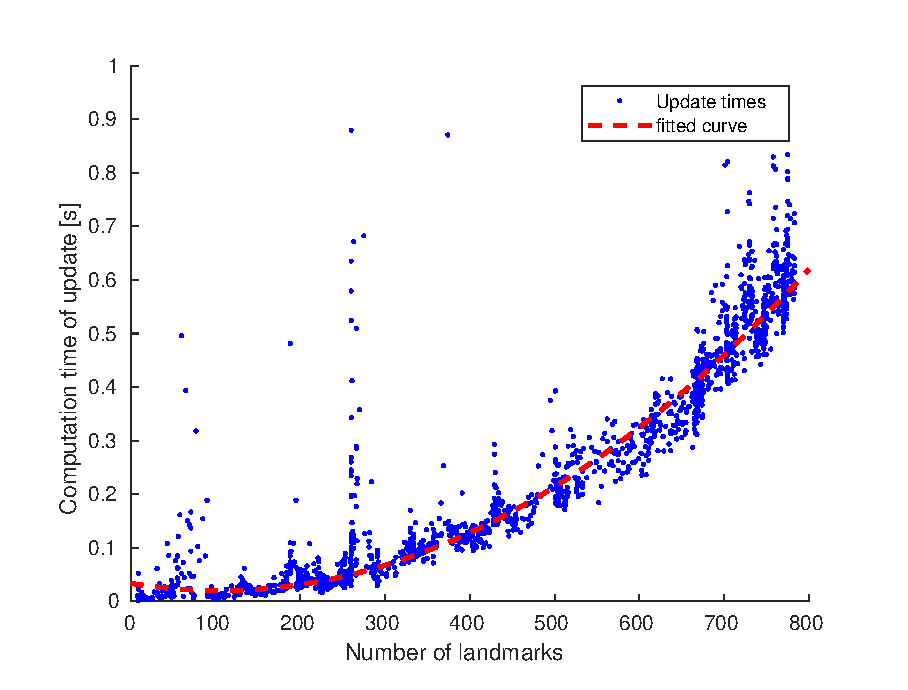
\includegraphics[width=0.7\textwidth]{plots/a3/update-time-vs-landmarks}
\caption{Update time vs landmarks}
\label{fig:update_time_landmarks}
\end{figure}



\subsubsection{Computational Performance of EKF-SLAM}
EKF-SLAM has been critizised for a variety of reasons in the literature, and one of the issues often brought up is computational performance as the map grows. Keeping the computation time down is of paramount importance in the online SLAM problem where delayed updates are not acceptable. In fact, each timestep of EKF-SLAM has a computational complexity of $\mathcal{O}(n^2)$ in the number of detected landmarks\cite{divideandconq}, something our implementation confirms. When tuned to provoke lots of landmark detections (around 800), the update step of the Kalman filter takes quadratic time, as shown in figure \ref{fig:update_time_landmarks}. These results show that in large environments, EKF-SLAM alone fails to meet the time-requirements for online SLAM.
\begin{figure}
    \centering
    \begin{subfigure}{0.45\textwidth}
        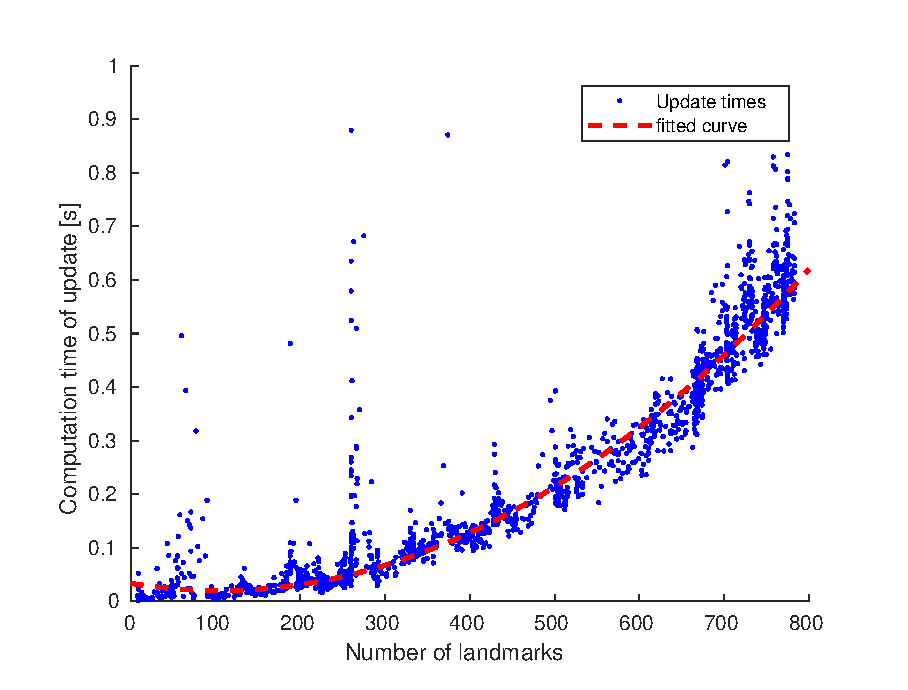
\includegraphics[width=\textwidth]{plots/a3/update-time-vs-landmarks}
        \caption{Update time vs landmarks}
        \label{fig:update_time_landmarks}
    \end{subfigure}%
~
    \begin{subfigure}{0.45\textwidth}
        \includegraphics[width=\textwidth]{plots/a3-real-results-bg}
        \caption{Trajectory overlayed Google Maps}
        \label{fig:results_bg}
    \end{subfigure}
\end{figure}

\subsubsection{Measurement Clutter}
After a successful run of the EKF-SLAM algorithm on the Victoria Park dataset, we typically find around 300 landmarks. For this reason, we have speculated that not all these landmarks correspond to actual trees, even though that is what they are supposed to represent. One of the reasons for this is landmarks being doubly registered due to the JCBB algorithm not making the proper associations. But another reason that must not be overlooked is the effect of clutter in the measurement data. The laser data in the dataset has been processed to only contain measurements that match a certain tree-profile\cite{victoria}, however no classification algorithm is perfect and we speculate that a lot of the measurements are spurious and should be regarded as clutter. This partly stems from the fact that a lot of the detected landmarks happen to appear inside the six-lane intersection to the east of Victoria Park, as can be seen in figure \ref{fig:results_bg}. In our experiments, the effect of clutter has not been significant, and spuriously detected landmarks have not had a noticeable impact on SLAM performance. It might however become problematic for longer operation times and larger maps. Keeping the number of landmarks down is essential to successfully apply EKF-SLAM in an online situation. In addition, wrongly registered landmarks might lead to spurious associations in the future and ultimately worsen the tracking performance. In our implementation, all unassociated measurements are initialized as new landmarks and never face the possibility of removal, there are however techniques to remove landmarks which have low probability of corresponding to an actual real life feature. One possibility would be to employ something akin to the IPDA mentioned in \ref{sec:a1} since it has a concept of target existance that in a SLAM context could be used to discriminate false landmarks.

\subsubsection{Choice of JCBB CI Bounds with Implication on Robustness}
The JCBB algorithm operates with two confidence intervals, one for joint and one for individual compatibility. The Mahalonobis distances of both joint and individual compatibility are gated with these confidence intervals to determine whether to move on with a given hypothesis.\cite{jcbb} In the Victoria Park dataset, we found that the choice of large confidence intervals ($\alpha_1 = 10^{-5}$ and $\alpha_2 = 10^{-3}$ for joint and individual respectively) gave perfectly satisfactory association speed on the dataset, however when EKF-SLAM was rerun on the generated map with a slight offset in orientation of $6^\circ$ (such a situation could appear naturally from disturbances such temporary loss of sensor data), the JCBB algorithm wound up in an almost complete stall after a few hundred timesteps, likely because all hypothesis were regarded as more equally likely due to the offset, making the algorithm unable to reduce the search tree and single out the best association in reasonable time. Choosing tighter confidence intervals on the other hand, with $\alpha = 0.1$ for both joint and individual, many more associations were gated out and hence only the most promising hypotheses were considered, ultimately leading to reasonable execution times. In the end, this made the rerun on the previously built map perfectly possible with no significant slow-down. This result shows how the choice of these confidence intervals is detrimental to the robustness of EKF-SLAM and crucial for online SLAM as a small disturbance can cause the JCBB algorithm to fail to find associations within reasonable time.


